\documentclass[11pt]{article}

% === Page Layout ===
\usepackage[a4paper, margin=1in]{geometry}

% === Packages ===
\usepackage{graphicx}
\usepackage{comment}
\usepackage{fancyhdr}
\usepackage{enumitem}
\usepackage{amsmath, amssymb}

% === Header/Footer Setup ===
\pagestyle{fancy}
\fancyhf{}
\fancyhead[L]{Multimodal Deep Learning}
\fancyhead[R]{Answer Sheet 5}
\fancyfoot[C]{\thepage}

\begin{document}

% === Title Information ===
\begin{center}
    {\Large \textbf{Multimodal Deep Learning}} \\ [0.3em]
    {\large \textbf{Answer Sheet 5}} \\ [0.3em]
    \large Date: June 17, 2025
\end{center}

\vspace{1cm}

\subsection*{Exercise 1: Graph representations}

\begin{figure}[h]
    \centering
    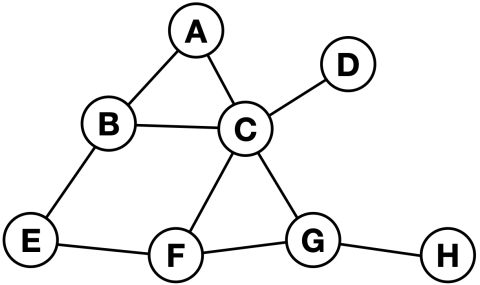
\includegraphics[width=7cm]{graph.png}
\end{figure}

\noindent
Given is above's graph with the vertices \(\mathcal{V}\) = \{\textbf{A, B, C, D, E, F, G, H}\}.

\begin{enumerate}[label=(\alph*)]
    \item {
        Write down its representation as list of edges \(\mathcal{E}\). \\
        \textbf{Answer: } \(\mathcal{E}\) = \{\textbf{(A,B), (A,C), (B,E), (B,C), (C,D), (C,F), (F,G), (G,H)}\}
    }
    \item {
        Write down its representation as the adjacency matrix \(\mathcal{A}\). \\
        \textbf{Answer: } 
        \[
            \mathcal{A} = \begin{bmatrix}
                0 & 1 & 1 & 0 & 0 & 0 & 0 & 0 \\ 
                1 & 0 & 1 & 0 & 1 & 0 & 0 & 0 \\ 
                1 & 1 & 0 & 1 & 0 & 1 & 1 & 0 \\ 
                0 & 0 & 1 & 0 & 0 & 0 & 0 & 0 \\ 
                0 & 1 & 0 & 0 & 0 & 1 & 0 & 0 \\ 
                0 & 0 & 1 & 0 & 1 & 0 & 1 & 0 \\ 
                0 & 0 & 1 & 0 & 0 & 1 & 0 & 1 \\ 
                0 & 0 & 0 & 0 & 0 & 0 & 1 & 0
            \end{bmatrix}
        \]    
    }
\end{enumerate}

\subsection*{Exercise 2: Graph scaling}

\noindent
Assume a social graph of 1,000,000 members (nodes) and that each node is connected to 200
randomly selected other nodes.

\begin{enumerate}[label=(\alph*)]
    \item {
        How large is the adjacency matrix of this graph? \\ 
        \textbf{Answer: } The size of the adjacency matrix \(\mathcal{A}\) is \((10^6, 10^6)\), which contains \(10^6 \times 10^6 = 10^12\) elements -- a very sparse matrix.  
    }
    \item {
        How many entries of the adjacency matrix are non-zero? \\
        \textbf{Answer: } There will be only \(200 \times 10^6 = 2 \times 10^8\) entries, which is equivalent to 0.02\%.
    }
    \item {
        Given a random node, estimate how many hops are required until 50\% of the network can be reached? \\ 
        \textbf{Answer: } With Erdős-Rényi model, a.k.a random graph theory, given \(k = 200\) and \(h\) is the number of hops.
        Hence,
        
        \[
            R(h) = 1 + \sum_{i=0}^{h-1} k(k-1)^i \approx 1 + k \cdot \frac{(k-1)^h - 1}{k-2}
        \]

        As \(R(h) =\) 50\% of 1,000,000. \\ 
        Therefore, 
            \begin{align*}
                500000 &= 1 + 200 \times \frac{199^h - 1}{198} \\
                \therefore \quad h &\approx 2.48 \approx 2.5 \ \text{hops} 
            \end{align*}
    }
    \item Why may this estimation not hold in real-world social graphs?
    \item How would above’s scaling behavior affect the application of graph convolutional neural
networks?
\end{enumerate} 

\end{document}